\chapter{Synchronisation}
\label{section:synchronisation}


In \Peano, every rank holds a set of spacetrees.
This set is held by the singleton \texttt{peano4::parallel::SpacetreeSet}.
Rank 0 serves as \emph{global master rank}, i.e.~instructs all other ranks what
to do. 
For this, is sends out activation messages.


Once we have made a decision which step to run, and once this information is
broadcasted to all other ranks, every rank creates a \emph{traversal observer}.
This observer is not yet bound to a particular tree. 
It serves as \emph{prototype}.


Next, the spacetree set tells all of its trees on all of the ranks to run
through the tree. 
Upon startup, each tree creates its own clone of the observer prototype and
passes its the tree number.
The clone is destroyed at one point after the traversal has completed.


Even though the sets are synchronised throug their startup messages with each
other, 
the actual tree traversals are not synchronised.
They run on different ranks, and maybe on different threads---you don't know.
As a result, there's no temporal order between the clones of the prototypes and
their destruction.
Some observer objects for some trees might be destroyed already again before
others are even created.
There's not a lot of synchronisation.


Obviously, some codes require synchronisation in some steps.
Classic examples are the reduction of global quantities or the responsibility to
create meta files over all snapshots written.
There's different ways how to realise this:


\subsection*{One global shared object per rank}

One of the simplest solution is to create one object per rank in your main
function as a global variable.
The individual observers know this global variable and call functions on it.
This ensures that all observer clones work against the same global variable.
In the main function, you issue the \texttt{traverse} calls on the spacetree
set, i.e.~you know exactly when all rank-local traversals have terminated. 
Therefore, you can reduce the global objects manually (within your main).
\texttt{tarch::mpi::Rank} offers routines to do this in a transparent, fast way
without blocking other data exchange in a massively parallel environment.


\begin{center}
 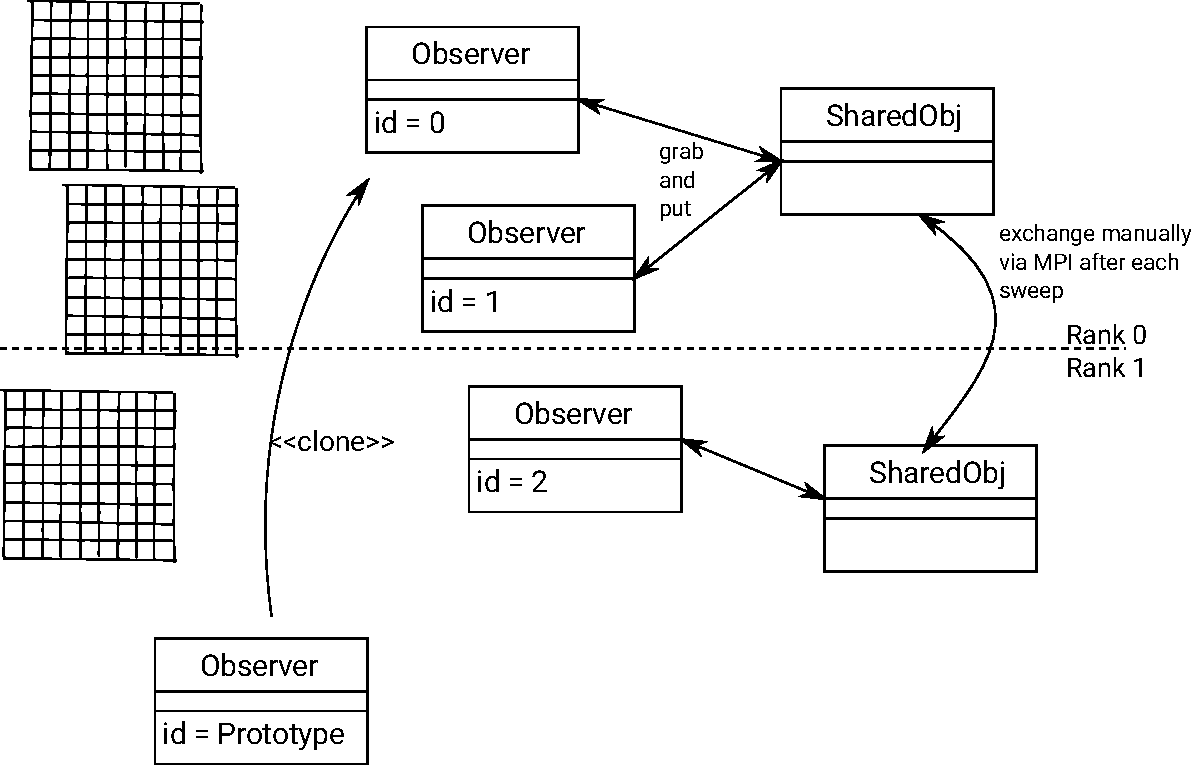
\includegraphics[width=0.75\textwidth]{37_synchronisation/synchronisation-01.pdf}
\end{center}


Here are some pros and cons of this solution:
\begin{itemize}
  \item[+] It is very simple to program;
  \item[+] You have explicit control over when data is reduced from threads into
  the rank-global shared object, and when the individual ranks actually reduce
  their data globally.
  \item[+] You don't have to care how observer clones see a global data
  representation. They always work against a global variable and thus see a
  consistent state always.
  \item[+] If global information expires after an iteration, you can realise
  this ``forget''-mechanism explicitly within your main. Even though you don't
  know when clones are created or destroyed, you know on the main-loop level per
  rank when all local traversals are done or start up.
  \item[-] If the individual observers reduce data into the shared object
  frequently, you have to synchronise manually and you might run into
  performance/locking issues.
\end{itemize}


\begin{remark}
 \ExaHyPE's solvers realise this pattern.
 All the flux functions and Riemann solvers do not exchange data with each
 other---besides the global time step size if we have adaptive time
 stepping---so this seems to be a 
\end{remark}



\subsection*{Global overview file}

Assume each observer writes its own data or file, i.e.~when we clone an observer
(or wen we call its \texttt{beginTraversal}; either option works), we set up all
variables locally.
No race conditions can occur.
When we close the observer, we open a global file in append mode and add a link
to our own data dump.


\begin{center}
 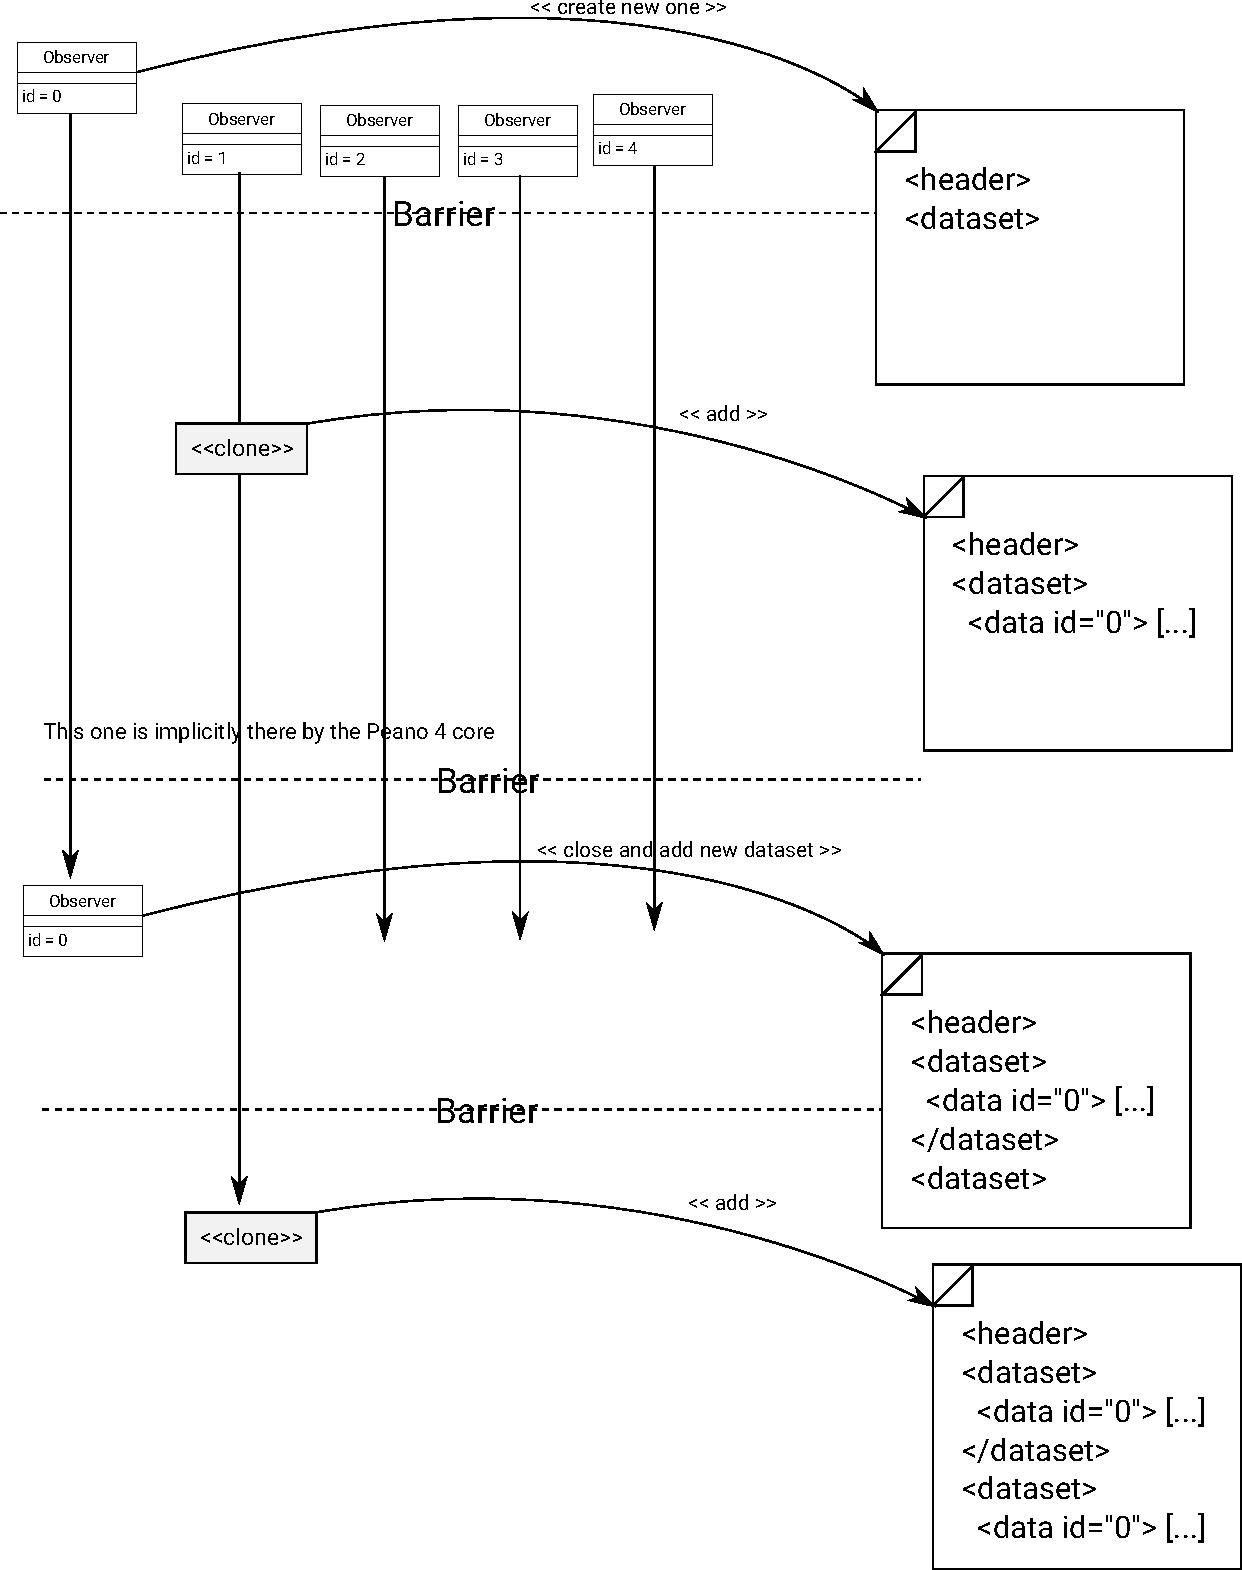
\includegraphics[width=0.75\textwidth]{37_synchronisation/synchronisation-02.pdf}
\end{center}



If we follow this pattern, we get a big blurb of a meta (overview) file and if
we run the code multiple times, we get a meta file which grows and grows and
grows.
So it is clear we have to implement two special rules for tree 0 which is the
only tree we know.
I propose to realise this special knowledge within the clone's construction
where we have the tree number as argument directly.


So if an observer is cloned for tree zero for the very first time (use a static
bool within the function), then we know that this is the very first tree
traversal in the whole run where the global spacetree is traversed.
At this point, it doesn't yet exist. Only the global root plus its children are
there.
So we delete the meta file and create a new one.
This means we are all prepared for all the new data.


Every time we create a new clone for tree number 0, we can know that we've just
kicked off a new traversal over our set of spacetrees.
Consequently, we can add a remark into our meta data file that we are now
starting a new set of dumps.


While this scheme so far is straightforward, it introduced a race condition: 
We cannot be sure that subsequent creations of tree number 0 happen before other
trees create their observer for a new grid sweep.
This is, tree 10 and 11 might have written their dump (and consequently
appended their local data file reference to the global meta file) before we even
start to kick off rank 0's dump.


 
Hence, it is important that we add a barrier to such a dump routine and
protect it via a semaphore.
As we don't really know in which order the observers are cloned, and as we have
to assume that clones are created serially, it is not a good idea to have either
of them in the clone's constructor.
Instead, I recommend that you use your observer's
\texttt{beginTraversal} event.
As we know that the observer creation is kind of lockstepped as all ranks
receive the startup call around the same time.
So it is safe to add a barrier before the routine writing to the meta file
(that's the plotter's constructor, e.g.) for all ranks besides 0.
For 0, it is important to place this barrier after the write into the metafile.
This way, the temporal order of accesses to the metafile is fine.
Next, we protect all accesses to the write via an MPI semaphore
(\texttt{tarch::mpi::BooleanSemaphore}).
Actually, there's no need to protect 0. 
For the other trees, a semaphore however is a must.




\begin{remark}
 \Peano's file dumps from the toolbox work this way.
 These are also the building blocks \ExaHyPE\ uses.
\end{remark}


\subsection*{One data copy per observer}

\marginpar{This is not complete yet}

Let each prototype have a prototype implementation of the shared data.
Let each observer have a standard attribute.
When we clone the prototype per rank, we can also clone this attribute.
Each observer now can work against its local copy of the attribute
independently.
The observers are totally independent of each other and we have, by definition,
no races.


Each observer clone has an operation \texttt{endTraversalOnRank} that
is invoked after the travesal.
This is where we have to restrict data globally.
We know that one tree will always exist and that's tree number 0. 
So we make \texttt{endTraversalOnRank} on all other trees reduce their data


\begin{remark}
 Have to continue to write this one. Its not complete yet!
\end{remark}


\begin{remark}
 \Peano's built-in \texttt{TraversalVTKPlotter} works this way. 
 \ExaHyPE's solvers realise this pattern.
\end{remark}

